%----------------------------------------------------------------------------------------
%    PACKAGES AND THEMES
%----------------------------------------------------------------------------------------
\documentclass[aspectratio=169,xcolor=dvipsnames]{beamer}
\makeatletter
\def\input@path{{BeamerTemplate/theme/}}
\makeatother
\usetheme{CleanEasy}
\usepackage[utf8]{inputenc}
\usepackage{lmodern}
\usepackage[T1]{fontenc}
\usepackage{fix-cm}
\usepackage{amsmath}
\usepackage{mathtools}
\usepackage{listings}
\usepackage{xcolor}
\usepackage{hyperref}
\usepackage{graphicx}
\usepackage{booktabs}
\usepackage{tikz}
\usetikzlibrary{positioning, shapes, arrows, calc, decorations.pathreplacing, arrows.meta, backgrounds, patterns, overlay-beamer-styles}
\usepackage{etoolbox}

%----------------------------------------------------------------------------------------
%    LAYOUT CONFIGURATION
%----------------------------------------------------------------------------------------
% Code listing style
\lstset{
  basicstyle=\ttfamily\small,
  keywordstyle=\color{blue},
  commentstyle=\color{green!60!black},
  stringstyle=\color{red},
  showstringspaces=false,
  breaklines=true,
  frame=single,
  rulecolor=\color{black!30},
  backgroundcolor=\color{black!5},
  numbers=left,
  numberstyle=\tiny\color{black!70},
  numbersep=5pt
}

% Colors for code boxes
\definecolor{codebg}{HTML}{1E1E2E}
\definecolor{codetext}{HTML}{CDD6F4}
\definecolor{codegreen}{HTML}{A6E3A1}
\definecolor{themeblue}{rgb}{0.05, 0.15, 0.35}

%----------------------------------------------------------------------------------------
%    TITLE PAGE
%----------------------------------------------------------------------------------------
\title[AI-Assisted Learning]{How to Learn Course Content Using AI}
\author[M. Jeon]{Minseok Jeon}
\institute[DGIST]{PLX Lab\\DGIST}
\date{2026}
\titlegraphic{
  \begin{tikzpicture}[remember picture, overlay]
  \end{tikzpicture}
}

%----------------------------------------------------------------------------------------

\begin{document}

\begin{frame}[plain]
  \titlepage
\end{frame}

\begin{frame}[plain]{Contents}
  \tableofcontents
\end{frame}

% ══════════════════════════════════════
\section{Motivation}
% ══════════════════════════════════════

\begin{frame}{Why Use AI for Learning?}
  \begin{itemize}
    \item Traditional learning: attend lecture $\rightarrow$ read notes $\rightarrow$ study alone
    \item \textbf{Problem:} When stuck, you have to wait for office hours or search online
    \item \textbf{AI-assisted learning:} Get instant, detailed explanations anytime
  \end{itemize}

  \vspace{1em}
  \begin{block}{Key Idea}
    Use AI as your \textbf{personal course tutor} that has access to all your course materials.
  \end{block}
\end{frame}

\begin{frame}{What Can AI Help With?}
  \begin{columns}[T]
    \begin{column}{0.48\textwidth}
      \textbf{Concept Understanding}
      \begin{itemize}
        \item Explain each slide in detail
        \item Break down complex topics
        \item Provide additional examples
      \end{itemize}

      \vspace{1em}
      \textbf{Coding Practice}
      \begin{itemize}
        \item Generate executable code
        \item Add detailed comments
        \item Create variations to explore
      \end{itemize}
    \end{column}
    \begin{column}{0.48\textwidth}
      \textbf{Deep Dive \& Verification}
      \begin{itemize}
        \item Cross-check slide content
        \item Find missing details
        \item Clarify ambiguities
      \end{itemize}

      \vspace{1em}
      \textbf{Self-Assessment}
      \begin{itemize}
        \item Generate quizzes
        \item Test your understanding
        \item Identify weak areas
      \end{itemize}
    \end{column}
  \end{columns}
\end{frame}

% ══════════════════════════════════════
\section{Tools}
% ══════════════════════════════════════

\begin{frame}{Tools You Need}
  \begin{center}
    \begin{tikzpicture}[
      box/.style={draw=themeblue, fill=MutedBlue, rounded corners=8pt,
                  minimum width=4.5cm, minimum height=1.8cm, align=center,
                  font=\bfseries},
      arr/.style={-{Stealth[length=6pt]}, thick, themeblue}
    ]
      \node[box] (vscode) at (0,0) {Visual Studio Code \\ \normalfont\small Code editor};
      \node[box] (claude) at (7,0) {Claude Code \\ \normalfont\small AI assistant (extension)};
      \draw[arr, <->] (vscode) -- node[above, font=\small] {integrated} (claude);
    \end{tikzpicture}
  \end{center}

  \vspace{1em}
  \begin{itemize}
    \item \textbf{Visual Studio Code}: Free code editor by Microsoft
    \item \textbf{Claude Code}: AI coding assistant by Anthropic
    \item Claude Code runs as an extension inside VS Code
  \end{itemize}
\end{frame}

\begin{frame}{Requirements}
  \begin{columns}[T]
    \begin{column}{0.48\textwidth}
      \textbf{Software}
      \begin{itemize}
        \item Visual Studio Code
        \item Node.js (version 18+)
        \item Claude Code (npm package)
        \item Claude Code VS Code extension
      \end{itemize}
    \end{column}
    \begin{column}{0.48\textwidth}
      \textbf{Account}
      \begin{itemize}
        \item Claude.ai account
        \item Claude Pro or Max subscription
        \item Stable internet connection
      \end{itemize}
    \end{column}
  \end{columns}
\end{frame}

% ══════════════════════════════════════
\section{Setup}
% ══════════════════════════════════════

\begin{frame}{Step 1: Install Visual Studio Code}
  \begin{enumerate}
    \item Go to \url{https://code.visualstudio.com/}
    \item Download for your OS (macOS / Windows)
    \item Install:
      \begin{itemize}
        \item \textbf{macOS}: Open \texttt{.dmg}, drag to Applications
        \item \textbf{Windows}: Run \texttt{.exe} installer, check ``Add to PATH''
      \end{itemize}
    \item Launch VS Code to verify
  \end{enumerate}
\end{frame}

\begin{frame}{Step 2: Install Node.js}
  \begin{enumerate}
    \item Go to \url{https://nodejs.org/}
    \item Download the \textbf{LTS} version (v20+ recommended)
    \item Install and verify:
  \end{enumerate}

  \vspace{0.5em}
  \begin{center}
    \colorbox{codebg}{%
      \parbox{0.6\textwidth}{%
        \texttt{\textcolor{codegreen}{\$ node --version}}\\
        \texttt{\textcolor{codetext}{v20.x.x}}
      }%
    }
  \end{center}

  \vspace{0.5em}
  \begin{alertblock}{Note}
    Node.js is required for installing Claude Code via npm.
  \end{alertblock}
\end{frame}

\begin{frame}{Step 3: Install Claude Code}
  \begin{enumerate}
    \item Open your terminal (Terminal on macOS, Command Prompt on Windows)
    \item Install Claude Code globally:
  \end{enumerate}

  \vspace{0.5em}
  \begin{center}
    \colorbox{codebg}{%
      \parbox{0.7\textwidth}{%
        \texttt{\textcolor{codegreen}{\$ npm install -g @anthropic-ai/claude-code}}
      }%
    }
  \end{center}

  \vspace{0.5em}
  \begin{enumerate}
    \setcounter{enumi}{2}
    \item Authenticate by running \texttt{claude} (opens browser for sign-in)
    \item Verify with \texttt{claude doctor} --- all items should be green
  \end{enumerate}

  \vspace{0.5em}
  \begin{alertblock}{Warning}
    Do \textbf{not} use \texttt{sudo} (macOS) or run as Administrator (Windows).
  \end{alertblock}
\end{frame}

\begin{frame}{Step 4: Install Claude Code Extension in VS Code}
  \begin{enumerate}
    \item Open VS Code
    \item Open Extensions panel:
      \begin{itemize}
        \item macOS: \texttt{Cmd + Shift + X}
        \item Windows: \texttt{Ctrl + Shift + X}
      \end{itemize}
    \item Search for ``\textbf{Claude Code}''
    \item Install the official extension by \textbf{Anthropic}
    \item Sign in when prompted
  \end{enumerate}

  \vspace{0.5em}
  \begin{block}{Result}
    You now have VS Code with the Claude Code panel in the sidebar.
  \end{block}
\end{frame}

% ══════════════════════════════════════
\section{Learning Workflow}
% ══════════════════════════════════════

\begin{frame}{Overview: The Workflow}
  \begin{center}
    \begin{tikzpicture}[
      box/.style={draw=themeblue, fill=MutedBlue, rounded corners=6pt,
                  minimum width=3.2cm, minimum height=1.4cm, align=center,
                  font=\small\bfseries},
      arr/.style={-{Stealth[length=6pt]}, thick, themeblue}
    ]
      \node[box] (mat) at (0,0) {Course\\Materials};
      \node[box] (env) at (5,0) {VS Code +\\Claude Code};
      \node[box] (learn) at (10,0) {Deep\\Understanding};
      \draw[arr] (mat) -- (env);
      \draw[arr] (env) -- (learn);
    \end{tikzpicture}
  \end{center}

  \vspace{1em}
  \textbf{5 simple steps:}
  \begin{enumerate}
    \item Create a folder and place all course materials
    \item Open the folder in VS Code
    \item Type \texttt{/init} in Claude Code
    \item Set up Claude as your course tutor (with a prompt)
    \item Start asking questions
  \end{enumerate}
\end{frame}

\begin{frame}{Step 1: Prepare Your Course Folder}
  Create a folder and place \textbf{all} provided materials inside:

  \vspace{0.5em}
  \begin{center}
    \colorbox{codebg}{%
      \parbox{0.55\textwidth}{%
        \texttt{\textcolor{codegreen}{ProgrammingLanguages/}}\\
        \texttt{\textcolor{codetext}{~~lec1.pdf}}\\
        \texttt{\textcolor{codetext}{~~lec2.pdf}}\\
        \texttt{\textcolor{codetext}{~~lec3.pdf}}\\
        \texttt{\textcolor{codetext}{~~lec4.pdf}}\\
        \texttt{\textcolor{codetext}{~~lec5.pdf}}\\
        \texttt{\textcolor{codetext}{~~notes.pdf}}\\
        \texttt{\textcolor{codetext}{~~...}}
      }%
    }
  \end{center}

  \vspace{0.5em}
  \begin{exampleblock}{Tip}
    The more materials you provide (slides, notes, assignments), the better Claude can help.
  \end{exampleblock}
\end{frame}

\begin{frame}{Step 2: Open in VS Code}
  \begin{enumerate}
    \item Launch Visual Studio Code
    \item \textbf{File} $\rightarrow$ \textbf{Open Folder...} $\rightarrow$ Select your course folder
    \item Open the Claude Code panel in the sidebar
  \end{enumerate}

  \vspace{1em}
  \begin{center}
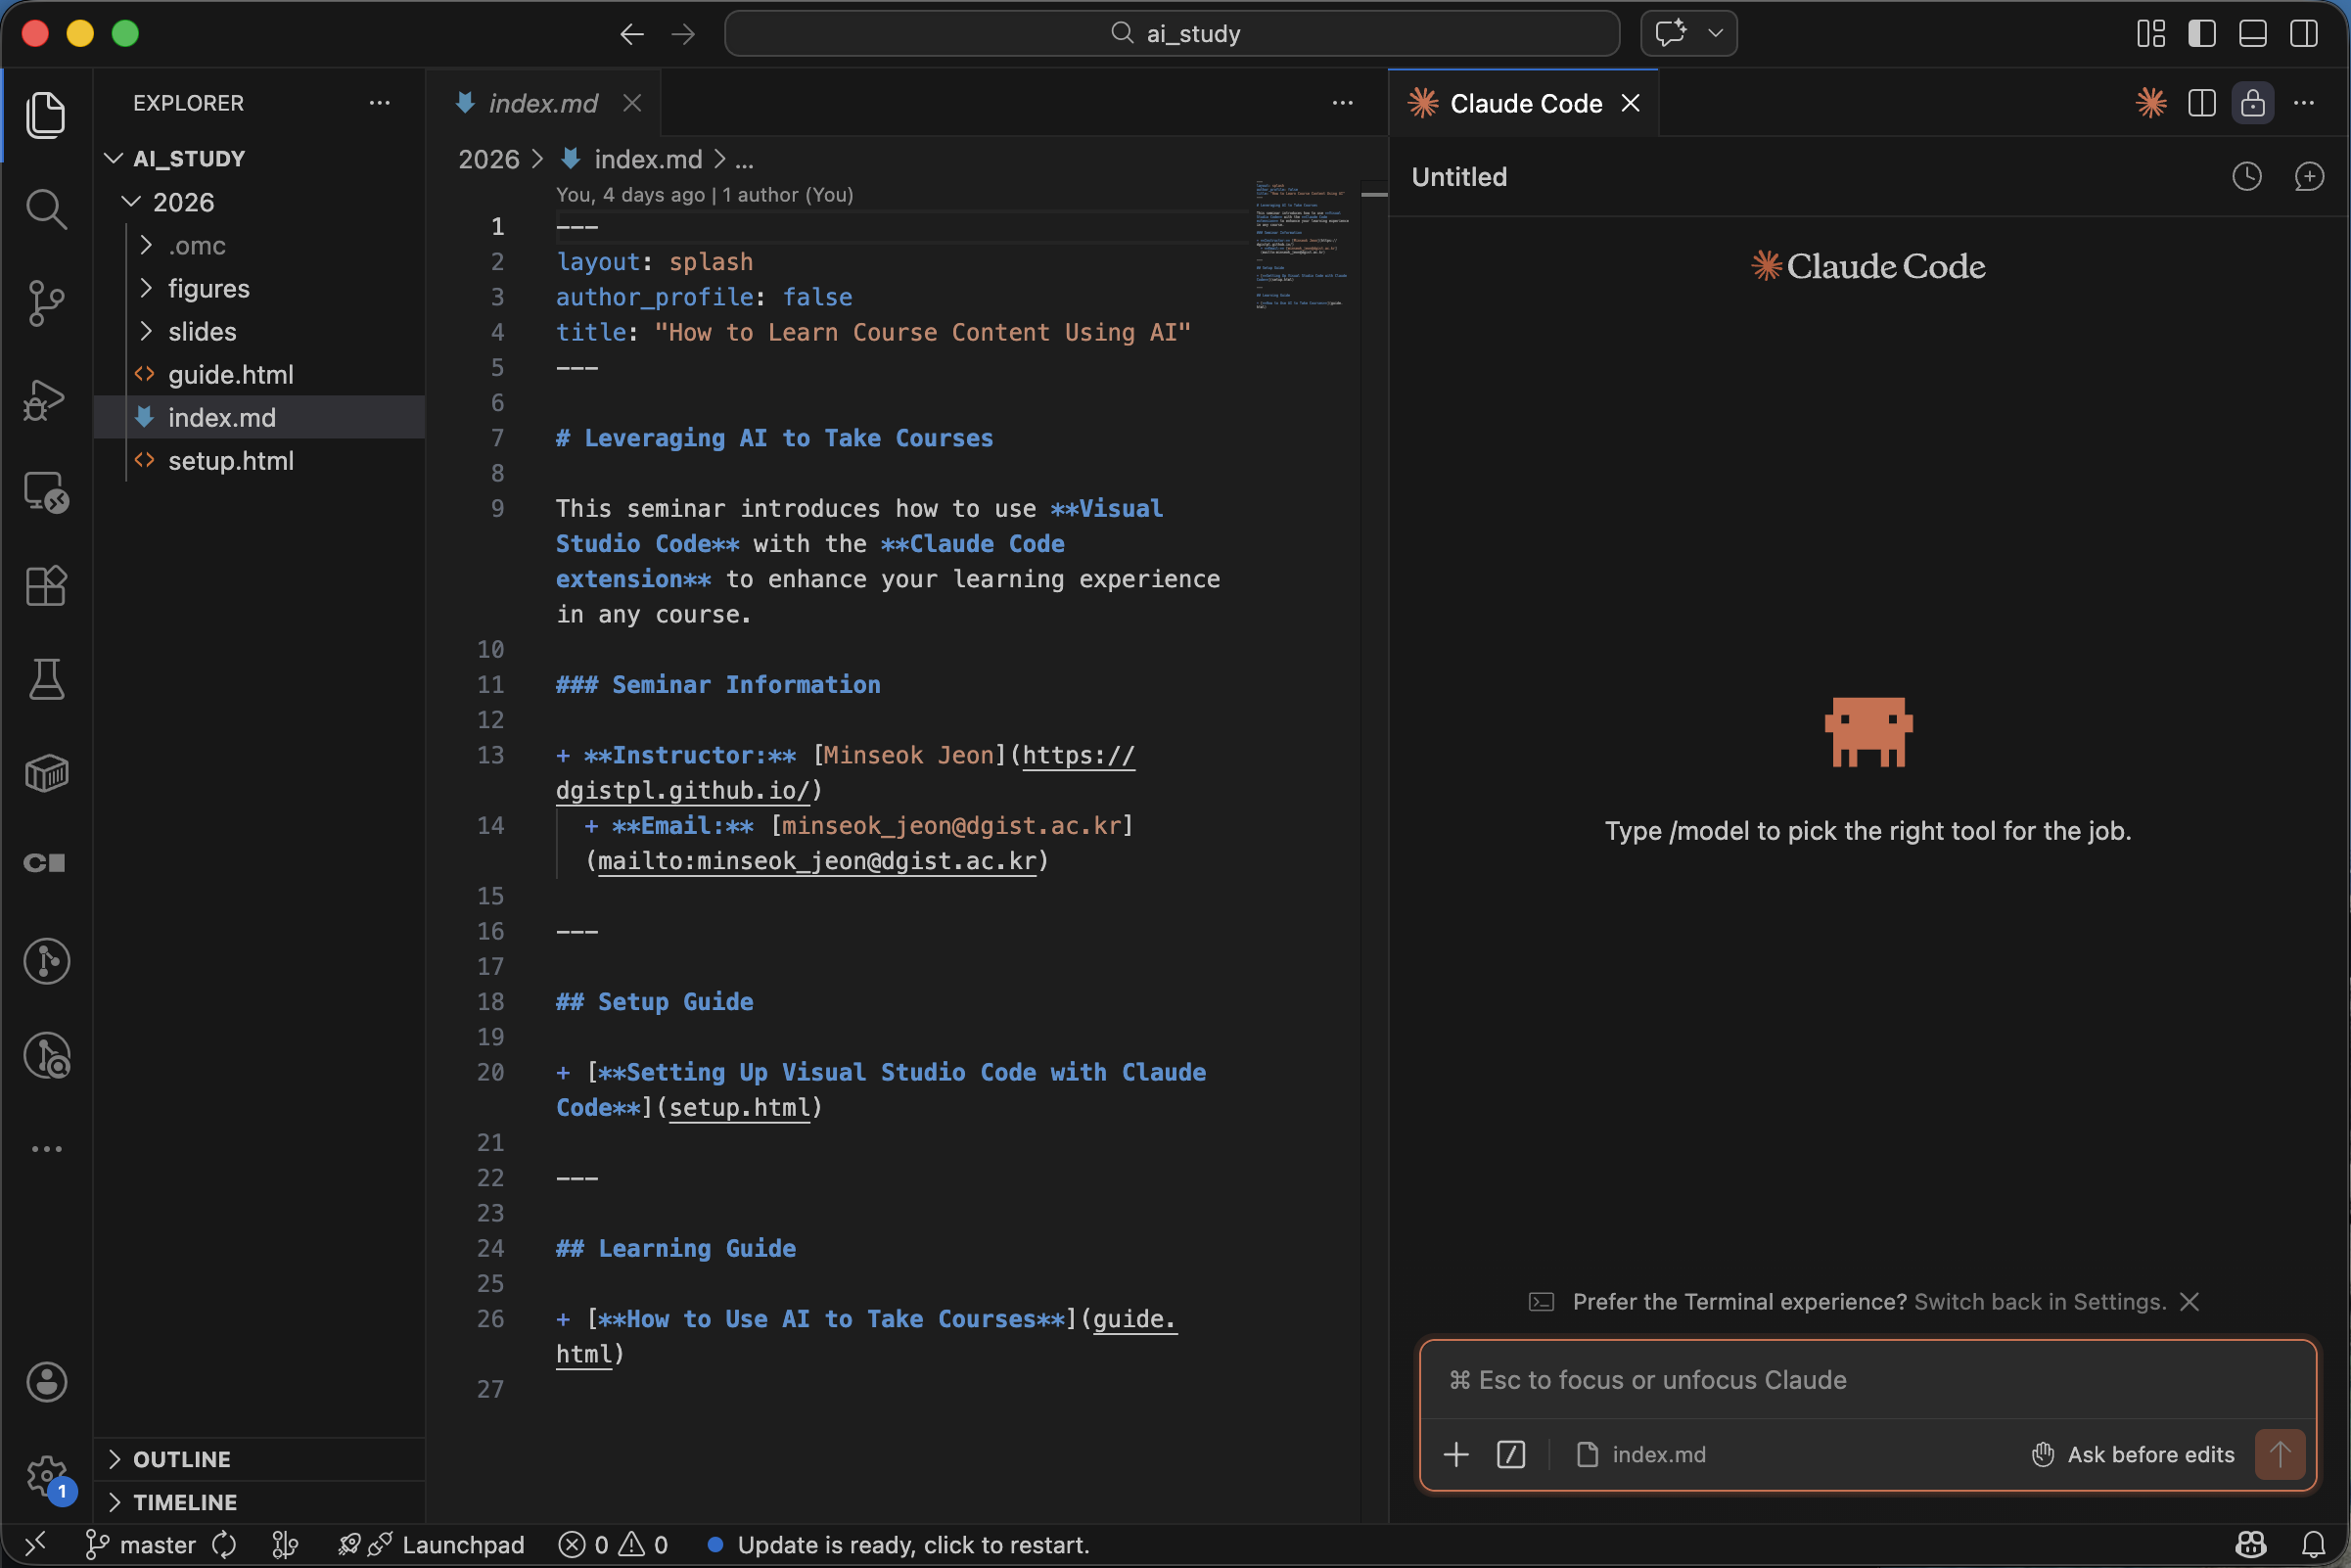
\includegraphics[width=0.5\textwidth]{../figures/vscode.png}
  \end{center}
\end{frame}

\begin{frame}{Step 3: Initialize with \texttt{/init}}
  In the Claude Code panel, type:

  \vspace{0.5em}
  \begin{center}
    \colorbox{codebg}{%
      \parbox{0.9\textwidth}{%
        \texttt{\textcolor{codegreen}{This folder contains all the materials for my course.
        Read all the files including .pdf and .md files.}}
      }%
    }
  \end{center}

  \vspace{1em}
  This creates a \texttt{CLAUDE.md} file that gives Claude context about your folder contents.
\end{frame}

\begin{frame}{Step 4: Set Up Your AI Tutor}
  Type the following prompt in Claude Code:

  \vspace{0.5em}
  \begin{center}
    \colorbox{codebg}{%
      \parbox{0.8\textwidth}{%
        \texttt{\textcolor{codegreen}{Context:}}\\
        \texttt{\textcolor{codetext}{Currently I am taking \{Course Name\} course}}\\
        \texttt{\textcolor{codetext}{where all the contents are provided in the folder.}}\\[4pt]
        \texttt{\textcolor{codegreen}{Role:}}\\
        \texttt{\textcolor{codetext}{You are the instructor of the course who will}}\\
        \texttt{\textcolor{codetext}{answer my questions about the course.}}\\[4pt]
        \texttt{\textcolor{codegreen}{Command:}}\\
        \texttt{\textcolor{codetext}{You need to answer my questions in detail}}\\
        \texttt{\textcolor{codetext}{and step-by-step.}}\\[4pt]
        \texttt{\textcolor{codegreen}{Format:}}\\
        \texttt{\textcolor{codetext}{If I request, save the illustration as a .md file.}}
      }%
    }
  \end{center}

  \vspace{0.5em}
  \small Replace \texttt{\{Course Name\}} with your actual course name.
\end{frame}

\begin{frame}{Step 5: Start Asking Questions!}
  \begin{center}
    {\Large You are now ready to learn.}
  \end{center}

  \vspace{1em}
  Claude can:
  \begin{itemize}
    \item Read your PDF slides and understand diagrams
    \item Provide detailed, step-by-step explanations
    \item Generate executable code examples
    \item Create quizzes to test your understanding
    \item Save explanations as \texttt{.md} files
  \end{itemize}
\end{frame}

% ══════════════════════════════════════
\section{Example Questions}
% ══════════════════════════════════════

\begin{frame}{Q1: Concept Check}
  \begin{block}{Goal}
    Understand each slide of a lecture in detail.
  \end{block}

  \vspace{0.5em}
  \textbf{Prompt:}
  \begin{center}
    \colorbox{codebg}{%
      \parbox{0.75\textwidth}{%
        \texttt{\textcolor{codetext}{For the first lecture (i.e., lec1.pdf),}}\\
        \texttt{\textcolor{codetext}{explain each slide in detail.}}
      }%
    }
  \end{center}

  \vspace{1em}
  \textbf{What Claude does:}
  \begin{itemize}
    \item Reads the PDF file
    \item Explains each slide one by one
    \item Provides context and background for each concept
  \end{itemize}
\end{frame}

\begin{frame}{Q2: Coding Practice}
  \begin{block}{Goal}
    Get executable code based on lecture content.
  \end{block}

  \vspace{0.5em}
  \textbf{Prompt:}
  \begin{center}
    \colorbox{codebg}{%
      \parbox{0.75\textwidth}{%
        \texttt{\textcolor{codetext}{For the third lecture (i.e., lec3.pdf),}}\\
        \texttt{\textcolor{codetext}{I need you to implement programs that I can}}\\
        \texttt{\textcolor{codetext}{execute. I need you to add detailed comments}}\\
        \texttt{\textcolor{codetext}{illustrating the role of each line.}}
      }%
    }
  \end{center}

  \vspace{1em}
  \textbf{What Claude does:}
  \begin{itemize}
    \item Creates runnable code files in your folder
    \item Adds line-by-line comments explaining each part
    \item You can run the code directly in VS Code's terminal
  \end{itemize}
\end{frame}

\begin{frame}{Q3: Deep Dive}
  \begin{block}{Goal}
    Challenge slide content and verify correctness.
  \end{block}

  \vspace{0.5em}
  \textbf{Prompt:}
  \begin{center}
    \colorbox{codebg}{%
      \parbox{0.75\textwidth}{%
        \texttt{\textcolor{codetext}{In page 15 of lec5.pdf, I guess the slide}}\\
        \texttt{\textcolor{codetext}{is wrong. The inference rule is missing some}}\\
        \texttt{\textcolor{codetext}{rules (the entire inference rules are}}\\
        \texttt{\textcolor{codetext}{provided in page 8).}}
      }%
    }
  \end{center}

  \vspace{1em}
  \textbf{What Claude does:}
  \begin{itemize}
    \item Cross-references page 15 with page 8
    \item Identifies missing or incorrect rules
    \item Provides the corrected version
  \end{itemize}
\end{frame}

\begin{frame}{Q4: Self-Assessment}
  \begin{block}{Goal}
    Test your understanding with quizzes.
  \end{block}

  \vspace{0.5em}
  \textbf{Prompt:}
  \begin{center}
    \colorbox{codebg}{%
      \parbox{0.75\textwidth}{%
        \texttt{\textcolor{codetext}{Based on the lecture notes and slides for}}\\
        \texttt{\textcolor{codetext}{lecture 5, give me a quiz for verifying my}}\\
        \texttt{\textcolor{codetext}{understanding of the lecture.}}
      }%
    }
  \end{center}

  \vspace{1em}
  \textbf{What Claude does:}
  \begin{itemize}
    \item Generates questions based on the lecture content
    \item Covers key concepts and potential exam topics
    \item Provides answers and explanations after you attempt
  \end{itemize}
\end{frame}

% ══════════════════════════════════════
\section{Tips}
% ══════════════════════════════════════

\begin{frame}{Tips for Effective Learning}
  \begin{enumerate}
    \item \textbf{Be specific with references}\\
      {\small Always mention the exact file and page number (e.g., ``page 15 of lec5.pdf'')}

    \vspace{0.5em}
    \item \textbf{Ask follow-up questions}\\
      {\small Don't stop at the first answer --- ask ``Why?'', ``Can you give another example?''}

    \vspace{0.5em}
    \item \textbf{Save important explanations}\\
      {\small Ask Claude to save as \texttt{.md} files to build your own study notes}

    \vspace{0.5em}
    \item \textbf{Run the code yourself}\\
      {\small Execute generated code in VS Code's terminal, modify and experiment}

    \vspace{0.5em}
    \item \textbf{Quiz yourself regularly}\\
      {\small Use self-assessment before exams to identify weak areas}
  \end{enumerate}
\end{frame}

% ══════════════════════════════════════
\section{Summary}
% ══════════════════════════════════════

\begin{frame}{Summary}
  \begin{center}
    \begin{tikzpicture}[
      scale=0.75, transform shape,
      box/.style={draw=themeblue, fill=MutedBlue, rounded corners=6pt,
                  minimum width=2.6cm, minimum height=1.2cm, align=center,
                  font=\small\bfseries},
      arr/.style={-{Stealth[length=5pt]}, thick, themeblue}
    ]
      \node[box] (s1) at (0,0) {Create\\Folder};
      \node[box] (s2) at (3.2,0) {Open in\\VS Code};
      \node[box] (s3) at (6.4,0) {\texttt{/init}};
      \node[box] (s4) at (9.6,0) {Set Up\\Tutor};
      \node[box] (s5) at (12.8,0) {Ask\\Questions};
      \draw[arr] (s1) -- (s2);
      \draw[arr] (s2) -- (s3);
      \draw[arr] (s3) -- (s4);
      \draw[arr] (s4) -- (s5);
    \end{tikzpicture}
  \end{center}

  \vspace{1.5em}
  \begin{itemize}
    \item Install: VS Code + Claude Code + Extension
    \item Place all course materials in one folder
    \item Use the structured prompt to set up your AI tutor
    \item Ask anything: concepts, code, deep dives, quizzes
  \end{itemize}

  \vspace{1em}
  \begin{center}
    \textbf{Setup Guide:} \url{https://dgistpl.github.io/courses/ai_study/2026/}
  \end{center}
\end{frame}

\begin{frame}[plain]
  \centering
  \Huge \textbf{Thank you!}

  \vspace{1cm}
  \normalsize
  \href{mailto:minseok_jeon@dgist.ac.kr}{minseok\_jeon@dgist.ac.kr}

  \vspace{0.5cm}
  \small
  \texttt{https://dgistpl.github.io/courses/ai\_study/2026/}
\end{frame}

\end{document}
